%========================================================================
\documentclass[10pt,a4paper]{report}
\usepackage[utf8x]{inputenc}
\usepackage{ucs}
\usepackage{amsmath}
\usepackage{amsfonts}
\usepackage{amssymb}
\usepackage{mathpazo}
\usepackage{makeidx}
\usepackage{xspace}
\usepackage{cooltooltips}
\usepackage{graphicx}

%========================================================================
\usepackage[pdftex]{hyperref}

%========================================================================
\hypersetup{
        colorlinks,%
	    citecolor=black,%
	    filecolor=black,%
	    linkcolor=black,%
	    urlcolor=blue
}

%========================================================================
\author{Alejandro Piad}
\title{\Huge Scientific Computing with Sci$\sharp$}

%========================================================================
% Index
\makeindex
\makeglossary

%========================================================================
% Commands
\newcommand{\cs}{C$\sharp$\xspace}
\newcommand{\sct}{\textbf{SciSharp}\xspace}
\newcommand{\code}[1]{\texttt{#1}}
\newcommand{\codelink}[1]{\code{#1}}
\newcommand{\typeref}[1]{{\codelink{#1}}\index{\codelink{#1}}}
\newcommand{\methodref}[2]{{\codelink{#2}}\index{\code{#1}!Method \codelink{#2}}}
\newcommand{\propertyref}[2]{{\codelink{#2}}\index{\code{#1}!Property \codelink{#2}}}
\newcommand{\cuttothechase}[2]{\marginpar{\small \mbox{$\Rightarrow$\\\hyperref[#1]{\texttt{#2}}}}}

%========================================================================
\begin{document}
%========================================================================

\maketitle
\tableofcontents
\listoffigures
\listoftables

%========================================================================
\chapter*{Preface}
\addcontentsline{toc}{chapter}{Preface}
 \sct\footnote{Although official named Sci$\sharp$, for ASCII compatibility
we will write the name as \sct, as it is the name used in the
rest of the documentation and all web-based content, to avoid using
the non-ascii $\sharp$ character, or worse, the \# character, which
is used to define anchors in URLs.} is a \cs library for scientific computing applications.
It contains a set of frameworks for a number of areas of scientific
computing, such as optimization, simulation, graph searching, 
probabilities and statistics, language processing, numerical algorithms,
computational geometry and number theory. It also provides tools for
testing and comparison of algorithms and for the generation of 
reports in several formats.

The main goal of \sct is to provide a set of tools for
the scientific community to develop algorithms in .NET for 
a very broad range of applications. Despite
being written entirely in \cs it aims to provide efficient
implementations, based on parallel, distributed and GPU programming
techniques.

Scientific computing is a very broad term which, for us, encompasses
the algorithms, frameworks and computational tools used by scientists in 
many different areas to solve domain-specific problems. It goes
from numerics to optimization, from statistics to machine learning,
from string matching to natural language processing, and so on.
We focus on a very narrow area of scientific computing, that is,
scientific computing for computer scientists. We say very narrow because
even if it is a big area (almost everything in computer science can
be fit into the definition of scientific computing -- notice the
word's resemblance), it does not contains specific tools or
techniques employed for instance by physicists, chemists, biologists 
and other scientists. That said, many of the tools provided
in \sct are of use for scientists of these areas. Physicists and
chemists often use numerical simulation techniques to model
processes, and biologists are among the most assiduous users
(and developers) of string matching techniques.

Although tailored for the scientist, \sct is also of use
for developers not much into science, but who want to provide some
``advanced'' features in their products which may require
techniques extracted from the computer science world.

This report describes the main functionalities built into
the library, and provides a guide for its use and extension.
It is by no mean a complete nor updated guide. \sct
is always changing, and the best place to find up to date and
extensive information on the nasty details of the library
is on its \href{http://scisharp.github.com}{website}.

The rest of the report is divided into chapters, one for each
of the \sct main \emph{namespaces}. Each chapter builds upon
one or more examples in a tutorial-like fashion. There are
of course many details that escape these examples. For some
of the most important details, footnotes or other indications will
be given.

%========================================================================
\section*{Prerequisites}
\addcontentsline{toc}{section}{Prerequisites}
%========================================================================

\sct is a library written in C\# for scientific computing. As
such, this manual considers on behalf of the reader a working
understanding both of the C\# language and the scientific topics
covered by the library. 

The algorithms and data structures implemented in the library
are in most cases well known in the scientific community.
In such cases, the first time a given algorithm, data structure
or any other important concept is mentioned in this manual, a
reference will be provided to the corresponding 
\href{http://en.wikipedia.org}{Wikipedia} page. All non-standard
modifications will be explained in detail proportional to
how strange or new is the given modification, and when possible
references will be provided from the corresponding papers or
websites.

%========================================================================
\section*{About the Source Code}
\addcontentsline{toc}{section}{About the Source Code}
%========================================================================

All code used throughout the manual is written in C\#, adhering
to the style used in by the developers of the library. Being a 
.NET library, all functionality can be used in any CLR compliant
language. Most the examples used in the manual are shipped
with the source code for the library. 
Source code will be formatted in \verb|monospace| font, with
the corresponding syntax highlight.

The \sct library has been designed following modern
design patterns and coding styles. Throughout the library we have
tried to be consistent with a unified style, which will be used in
the code examples for this manual. Being a scientific library, we
have tried also to provide support for some flavoured syntax styles
widely used in some scientific packages, such as Matlab and Octave.
We have also tried to supply a syntax as close as possible to that
used by academicians in the corresponding areas.

We have implemented this syntax sugar with heavy use of operators
overloading and other fluid interfaces techniques. This means 
that there are almost always two ways of doing things, with
the usual C\# syntax (dot notation and such) and with the flavoured
syntax which may involve using some strange operators and 
method names, in order to get a code that looks familiar
to the mathematician eye. 

We have designed the library this way because we feel it is
more natural for the scientist, but it could be weird for the
programmer used to the clean dot notation syntax. If you ever
feel uncomfortable using the flavoured syntax, you can
always find a way of doing the same thing using standard
C\# syntax. 

We particularly prefer the syntax sugar
\footnote{There is a common joke that says: \emph{Syntax sugar
causes cancer of the semicolon}.} whenever possible, because
we designed the library this way, it has become a
common language for the library developers, and in the code examples
you'll find it anywhere. In any case, in this manual we will
always provide hints of how to circumvent the syntax sugar
in favour of a more C\#-ist syntax.

%========================================================================
\section*{What this Manual Is Not}
\addcontentsline{toc}{section}{What this Manual Is Not}
%========================================================================

This manual is \textbf{not} a reference for algorithms and
data structures. You will not find implementation details for the
algorithms, nor proves of asymptotic complexity, or any other
theoretical details of the implemented tools, other than the very
basic definitions.

This manual does \textbf{not} explain which algorithm or technique
is better in which case, nor provides comparisons between algorithms 
other than (perhaps) some information about our particular implementation
that we think you may need to know. For instance, we will never say
that \emph{QuickSort} is faster than \emph{MergeSort} (well, I just did, but
that is not the point). We could say, however, that \textbf{our} \emph{QuickSort}
implementation is faster than \textbf{our} \emph{MergeSort} implementation.

You \textbf{will} find, however, links to
relevant places where you can start doing some research
about the techniques implemented. You can also look at the
source code in any moment, where you'll find all implementation
details you want (is all in there, isn't it?). Also, the
examples have been designed trying to choose interesting or at least
classic problems that can be solved using the corresponding
techniques. 

But always keep in mind that we are just giving you
a hammer, it is your choice how to use it: to build a house,
to bake some cookies, or to break someone's head. The examples
we provide will almost always be about house building, in fewer
cases about cooking, but \emph{almost} never about head smashing. 

%======================================================================== 
\chapter{Introduction}
\label{chap:introduction}

%======================================================================== 
\chapter{Numerics}
\label{chap:numerics}

%======================================================================== 
\chapter{Optimization}
\label{chap:optimization}

%======================================================================== 
\chapter{Machine Learning}
\label{chap:machine-learning}

%======================================================================== 
\chapter{Computational Geometry}
\label{chap:geometry}
 Computational geometry studies data structures and algorithms
useful to describe and solve geometrical problems. It goes from
computing basic geometrical magnitudes (distances, angles)
to the construction of efficient representations of geometrical
data for fast queries (e.g. nearest neighbours to a given point in space),
to the computation of geometrical relations between objects in
a metric space (visibility, connectivity, reachability).

In this chapter we will study a few basic geometrical problems,
and their computational solution, based on the tools available
on \sct. The \code{Geometry} namespace contains most of the 
geometry-related algorithms implemented in \sct. However, geometrically
related data structures, such as kd-trees and r-trees are found
under the \code{Collections} namespace instead.

\section{Convex Hull}\label{sec:convex-hull}

A
\cuttothechase{algorithm:graham-scan}{Graham's Scan}
\cuttothechase{algorithm:jarvis-march}{Jarvis March}
classic problem in computational geometry is the construction
of the convex hull of a set of points. Informally, the convex
hull is the minimum area convex polygon (in $R^2$) that surrounds the given set of points.
Extensions to $R^3$ and beyond are possible but considerably more complicated
than for $2$ dimensions.
If no three points are collinear, the convex hull
can be shown to be unique. In the other case, we can consider
to include or not the middle point(s), since the convex hull
area will remain the same. For simplicity, we will most of the time consider
this restriction to hold, since points with real coordinates
have a very small (probabilistically zero) chance of being collinear. 
However, the algorithms presented in this
section are oblivious to this restriction, and will simply drop (or not)
the middle point(s).

\begin{figure}
 \begin{center}
  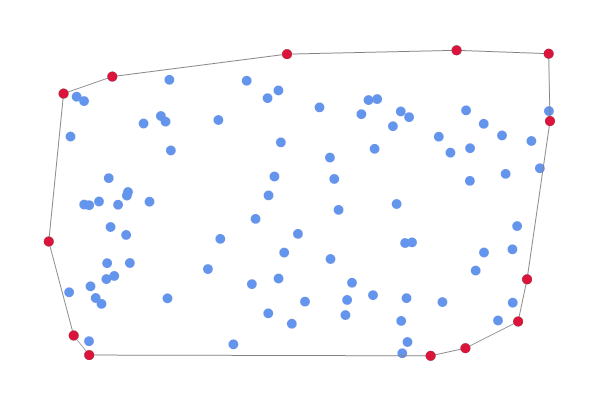
\includegraphics[width=0.8\textwidth]{Graphics/ConvexHullExample}
 \end{center}
 \caption[Convex Hull Example]{An example of the convex hull of a set of points in $R^2$.}
\end{figure}

Convex hulls seem to have no immediate application to real life problems.
However, they appear in the solution to many problems in 
CAD\footnote{Computer Aided Design} and computer simulation.

\subsection{Properties of Convex Hulls}\label{sub:convex-hull-properties}

Before diving into the algorithms we will discuss some basic 
properties of convex hulls, which allow us to build efficient
techniques to build them. 

First of all, there are a few points that will necessary be in the
convex hull. These are the \emph{extremal} points. The topmost,
leftmost, rightmost and bottommost points can be seen to fall
in this category easily. Note that some of these points can coincide.
For instance, the leftmost can also be the topmost or bottommost point.
For this reason, it is always safe to start building the convex at
one of these points. Again, if you have a tie, lets say, two points
with the minimum $x$, you'll need to break ties by choosing the 
upper (or lower) one. If both points also have the same $y$ then
they are the same point!

Since convex hulls are, well, convex, we can easily prove that
when walked in clockwise (or counter-clockwise) order, all points
turn to the same side. This will be the basic property used
by the Graham's scan algorithm (see the section \ref{sub:graham-scan}).
We can also prove that for every pair of adjacent points $x_i$, $x_{i+1}$ in the convex
hull (when taken clock-wise) the angle of the segment $\overline{x_i\,x_{i+1}}$
with respect to the horizontal (or any other reference line)
must be greater or equal than the angle
$\overline{x_i\,x_j}$ for any other $x_j$.
Otherwise the point $x_j$ would be outside the convex hull. This
property is key to prove to correctness of the Jarvis march algorithm
(see section \ref{sub:jarvis-march}).

\subsection{Graham's Scan}\label{sub:graham-scan}

\subsubsection*{Using Graham's Scan in \sct}\label{algorithm:graham-scan}

\subsection{Jarvis' March}\label{sub:jarvis-march}

\subsubsection*{Using Graham's Scan in \sct}\label{algorithm:graham-scan}

%======================================================================== 
\chapter{Language Processing}
\label{chap:language}
 The \texttt{Language} \emph{namespace} contains a framework
for the definition, parsing and processing of languages,
built around the concepts of grammars, automata and regular expressions.

%========================================================================
\section{Grammars}
%========================================================================

In the \texttt{Grammars} namespace you'll find an embedded DSL for
the definition of context-free attributed grammars. The basic class
is the \typeref{Grammar<T>}
class (and its non-generic counterpart \typeref{Grammar}).
This class is used to define a context-free grammar whose rule attributes
are defined by the generic parameter type.  

The grammar building is based on types that encapsulates the concepts
of non-terminal and terminal symbols, with defined operations for
the construction of production rules. On top of this classes, making
a heavy use of operator overloading and other fluid interfaces techniques
you'll find an embedded DSL which aims to provide a syntax as near as
possible to the EBNF notation used in the formal languages community.

To use this DSL, you only interact directly with the 
\typeref{Grammar<T>} class.

%------------------------------------------------------------------------
\subsection{Defining Symbols and Productions}
%------------------------------------------------------------------------

Let's begin with the construction of a parser for the very simple language
$L = \{ w = a^n b^n | n > 0 \}$. This is a classic context free language 
that will serve as base to show how to define symbols and productions.
Since we don't require the use of attributes, we'll be using the non-generic
\typeref{Grammar}{ScientificTools.Language.Grammars.Grammar} class.

We first need a \typeref{Grammar} instance,
which is created simply by calling its constructor.

\begin{verbatim}
var G = new Grammar();
\end{verbatim}

Now that we have a grammar, let's define the symbols (both non-terminal and terminals).
Non-terminal symbols are called \emph{rules}, while terminal symbols are called \emph{tokens}.
To define symbols we can use the methods \methodref{Grammar<T>}{Rule}
and \methodref{Grammar<T>}{Token} respectively.

\begin{verbatim}
var S = G.Rule("S");
var a = G.Token('a');
var b = G.Token('b');
\end{verbatim}

In the case of rules, you can pass in a name as an argument, just for debugging
purposes. In the case of tokens you need to provide either a simple \code{char}
or a \code{string} which will be the regular expression used to parse
the token. You can provide an optional name as well, but when you define
tokens using a \code{char} it is used for the name too.

Now it's time to define the production rules. For this very simple grammar there
is only very simple rule.
Productions are defined using the \code{\%=} operator
for definition (like the arrow $\rightarrow$ in EBNF)
\footnote{We would have prefer to use the \code{>>} operator, but unfortunately 
it can only be redefined with an \code{int} argument in \cs}, the \code{+} operator
for symbol concatenation
\footnote{In EBNF symbol concatenation is defined just by placing symbols
side of each other, but this is not possible in \cs}, 
and the \code{|} operator for branches, just like in EBNF.

\begin{verbatim}
S %= a + S + b | a + b;
\end{verbatim}

Now that the grammar is complete, we can test it by building a parser for it
or generating a lot of strings out of it (more on these topics later).

You could have skipped the definition of tokens \verb|a| and \verb|b|,
and use strings directly in the definition for the production, like this:

\begin{verbatim}
S %= "a" + S + "b" | "ab";
\end{verbatim}

This way you don't have to define dummy token just for a character or
a string. The \typeref{Grammar}{ScientificTools.Language.Grammars.Grammar} class
takes care of creating the token. Also, if you use the same string more than once,
you'll get the same \typeref{Token}{ScientificTools.Language.Grammars.Token`1} instance.
 
%======================================================================== 
\chapter{Statistics and Probabilities}
\label{chap:stats}

%======================================================================== 
\chapter{Simulation}
\label{chap:simulation}

%========================================================================
\newpage
\addcontentsline{toc}{chapter}{Index}

\begin{small}
 \printindex
\end{small}

%========================================================================
\end{document}
%========================================================================